\documentclass[a4paper,11pt]{article}

%=========================
% Les styles
%=========================
\usepackage{style-esi/french}	% Francise LaTeX
\usepackage{style-esi/td}
\usepackage{style-esi/licence}	% Affiche une licence dans le document
\usepackage{style-esi/exercice}
\usepackage{style-esi/consigne}
\usepackage{style-esi/listing}
\usepackage{style-esi/tutoriel}
\usepackage{style-esi/exemple}
%\marginsectiontrue
\usepackage{booktabs}
\usepackage{pifont}  



\definecolor{verylightgray}{rgb}{0.98,0.98,0.98}

\date{2018 -- 2019}
\siglecours{DEV1}
\libellecours{Laboratoires d'environnement}
%\libelledocument{TD 1 -- Prise en main de l’environnement }
\libelledocument{TD02 - Les bases de Linux }
\sigleprof{}



\begin{document}

\entete
\titre
\ccbysa{esi-dev1-list@he2b.be}
\lastedit


	%===================
	%  Contenu
	%====================
	\begin{tcolorbox}[blanker,
	before skip=10mm,after skip=10mm,
	borderline west={1mm}{-4mm}{lightgray},
	title=Objectifs, coltitle=black, fonttitle=\sffamily\bfseries\large]
	\`A l'issue de ce TD vous aurez acquis une connaissance basique de l'utilisation du syst\`eme Linux 
	et de son aide en ligne : man.   
	En particulier, les commandes \textbf{ls}, 
	\textbf{cd}, \textbf{pwd}, 
	\textbf{rm}, \textbf{rmdir}, 
	\textbf{mkdir}, \textbf{chmod}, 
	\textbf{mv} et \textbf{cat} 
	devront vous \^etre famili\`eres.  
	
	\par
	
	Vous serez aussi \`a l'aise avec le concept de \textbf{permissions} 
	sur les fichiers et vous saurez vous rep\'erer dans le \textbf{syst\`eme de fichiers}. 

	\end{tcolorbox}
	
	\tableofcontents

	%\newpage

%===================
\section{TD2 - Les bases de Linux}%\textbf{Consignes}:
%====================	
\begin{consigne}
\begin{itemize}
	\item Ce TD est accompagn\'e d'exercices \`a faire \textbf{avant} de venir au laboratoire.
\item Prenez bien note des r\'eponses aux exercices ainsi que de la fa\c con dont vous avez trouv\'e ces r\'eponses.

%
\end{itemize}
\end{consigne}


\begin{Tutoriel}{Se connecter \`a linux1}
	\textbf{Nous avons d\'ej\`a vu comment se
		connecter \`a linux1 !}

	
	
	Nous allons rapidement vous montrer comment configurer putty 
	si vous voulez l'adapter \`a vos envies. 
	
	
		\subparagraph{Configurer putty} 

\textcolor{white}{.} \par

\par

%\begin{itemize}
	\begin{steps}
	
	\item 
	
	Lancez \textit{putty}
	comme vous l'avez vu la semaine derni\`ere et entrez
	"\textit{linux1}" comme
	"\textit{Host Name}".
	
	
	\item \textbf{Avant} d'appuyez
	sur le bouton de connexion, vous pouvez par exemple
	apportez une modification :  
	
	
	\begin{steps}
		
		\item 
		
		Pour modifier l'aspect de votre console,
		faites un petit tour dans l'onglet "\textit{Window}" qui
		contient les cat\'egories "\textit{Appearance}" et
		"\textit{Colours}"
		
		
	\end{steps}
	
\end{steps}

	\end{Tutoriel}

		\subparagraph{FAQ} 

\textcolor{white}{.} \par

\par
\textbf{Et je vais devoir effectuer cette configuration \`a chaque fois ?}
\par

Nous avons une bonne et une mauvaise nouvelle pour vous. 
Commen\c cons par la bonne : il est possible de sauver une configuration.  
Pour cela, configurez \textit{putty} comme indiqu\'e plus haut 
mais avant de vous connecter, faites ceci :  

\par

\begin{itemize}
	
	\item revenez \`a la fen\^etre "\textit{Session}" ;
	\item 
	entrez un nom dans la champ de saisie "\textit{Saved Sessions}" 
	(par exemple : "\textit{Linux1}") ;
	
	\item Cliquez sur le bouton "\textit{Save}" ; 
	\item \`A pr\'esent, il suffira de double-cliquer sur la session "Linux1" pour ouvrir une connexion \`a linux1.
\end{itemize}
\textbf{Vous n'avez pas parl\'e d'une mauvaise nouvelle \'egalement ?}
\par

C'est vrai !
La session que vous venez de cr\'eer est sauv\'ee sur le poste de travail.
Si lors du prochain TD, vous vous connectez sur une autre machine, elle ne sera pas connue.
Vous devrez donc effectuer cette configuration une fois par machine utilis\'ee. 
(En fait, il est possible d'\'ecrire un petit fichier \`a stocker dans votre 
\verb@Z:@ avec la bonne configuration,
l'aide de putty vous explique comment faire \textbf{mais}, svp, ne perdez pas de temps \`a le faire maintenant!)   

\par


\subsection{Syst\`eme de fichiers, chemin absolu et relatif}\begin{quotation}
	\guillemotleft \textit{ Tout est relatif, et cela seul est absolu }\guillemotright . Auguste Comte.
\end{quotation}  
R\'eguli\`erement, il faut indiquer un endroit du syst\`eme de fichiers (par exemple pour y aller). 
D\'esigner simplement le nom du dossier ne suffit pas.  

\par

Un petit tour vers les points 10 \`a 14 du guide visuel sera peut-\^etre n\'ecessaire...  

\par



\begin{Exercice}{Dossier personnel}
	
%\textcolor{white}{.} \par

%\par
\begin{figure}[hbt]
	\begin{center}
		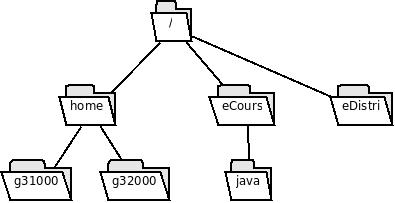
\includegraphics[width=0.8\linewidth,height=0.8\textheight,keepaspectratio=true]{/home/oxfam/Bureau/DEV1ARefaire/labo-cli-02/labo-cli-02/image/fs.jpeg}
	\end{center}
	
	\caption[Une partie d'un syst\`eme de fichiers]{Une partie d'un syst\`eme de fichiers}
\end{figure}

\begin{enumerate}
	
	\item 
	Pouvez-vous retrouver votre dossier personnel dans le syst\`eme de fichiers ?  
	
	\item 
	Entrez la commande \,\verb|pwd|\, (que fait-elle encore ?). 
	Comprenez-vous la notation qu'elle utilise pour la r\'eponse ?
	
\end{enumerate}

\end{Exercice}

\begin{Exercice}{Chemins absolus et relatifs}
%	\textcolor{white}{.} \par
	Parmi tous les chemins suivants, quels sont ceux qui sont 
	\textbf{relatifs} ?
	
	\begin{itemize} 
		
		\item[ \ding{"6F} ]  \verb@~/../g12345/td2@
		
		\item[ \ding{"6F} ]  \verb@/home/g12345/../g54321/Hello.java@
		
		\item[ \ding{"6F} ]  \verb@./tds/td2@
		
		\item[ \ding{"6F} ]  \verb@tds/td2/Hello.java@
		
		\item[ \ding{"6F} ]  \verb@~g12345/tds/td2@
		
	\end{itemize} 
\end{Exercice}


\begin{Tutoriel}{Chemin absolu}%					\textcolor{white}{.} \par
%\par
%
\begin{enumerate}	
	\item \'Ecrivez le chemin absolu d'un des fichiers que vous
	avez d\'ej\`a cr\'e\'e pour ce TD (Si vous n'en n'avez pas cr\'e\'e, 
	faites-le maintenant).  
	\item Visualisez le contenu de ce fichier en donnant un
	chemin absolu.
	\item Faites de m\^eme avec un fichier de votre voisin.
	
\end{enumerate}	
\end{Tutoriel}

%\clearpage

\begin{Tutoriel}{Raccourci}
%						\textcolor{white}{.} \par
%	
%	\par	
	Refaites les exercices pr\'ec\'edents en utilisant les raccourcis 
	\,\verb|~|\, et \,\verb|~g12345|\,.
	
	\par
\end{Tutoriel}


\begin{Tutoriel}{Chemins}
%						\textcolor{white}{.} \par
%	
%	\par	
	\begin{enumerate}
		
		\item Visualisez le contenu d'un des fichiers que vous avez d\'ej\`a cr\'e\'e pour ce TD en utilisant un chemin relatif.
		\item Faites de m\^eme avec un fichier du TD1. 
		\item Faites de m\^eme avec un fichier de votre voisin. 
		\item 
		Quel est le dossier d\'esign\'e par la notation suivante : \par
		\,\verb|/usr/bin/../../eCours/asm/../java|\, ?
		
	\end{enumerate}
\end{Tutoriel}



\subsection{Propri\'etaire et groupes}\begin{quotation}  
	\guillemotleft \textit{ La propri\'et\'e est un pi\`ege: ce que nous croyons poss\'eder nous poss\`ede }\guillemotright . 
	Alphonse Karr.  
\end{quotation}\begin{quotation}  
	\guillemotleft \textit{ La propri\'et\'e c'est le vol }\guillemotright . Pierre Joseph Proudhon.  
\end{quotation}  
Comme Linux est un syst\`eme partag\'e, il est important de parler de s\'ecurit\'e. 
Ici, on va se concentrer sur la s\'ecurit\'e au niveau des fichiers et r\'epondre aux questions suivantes :  

\par

\begin{itemize}
	
	\item \`A qui \textbf{appartient} un fichier ?
	\item \textbf{Qui peut faire} quoi avec un fichier ?
\end{itemize}

Mais pour commencer il faut d'abord comprendre la notion de \textit{propri\'etaire}
et celle de \textit{groupe}. 
Un retour vers les points 15 et 16 du guide visuel sera peut-\^etre n\'ecessaire...  

\par

\newpage
\begin{Tutoriel}{Propriétaire}%					\textcolor{white}{.} \par
%
%\par
\begin{enumerate}
	
	\item 
	Visualisez le propri\'etaire des fichiers de votre dossier personnel.
	
	\item 
	Visualisez le propri\'etaire des fichiers de votre dossier \verb@td1@.
	
\end{enumerate}	
	
	\end{Tutoriel}


\begin{Tutoriel}{Groupe}%					\textcolor{white}{.} \par%\par
\begin{enumerate}	
	\item Visualiser les groupes auxquels vous appartenez.
	\item Quel est votre groupe principal ? 
	\item Quels sont les groupes auxquels appartient votre professeur ?
	\item Avez-vous un groupe en commun avec lui ?
	\item Quel(s) groupe(s) Linux avez-vous en commun avec les autres \'etudiants de votre groupe ESI ?
\end{enumerate}	
		\end{Tutoriel}
	

\begin{Tutoriel}{Groupe}	
%					\textcolor{white}{.} \par
%
%\par
\begin{enumerate}
	
	\item Visualisez vos fichiers et d\'eterminez \`a quel groupe ils appartiennent.
	\item Cr\'eez un fichier de test et modifiez le groupe auquel il appartient.
\end{enumerate}
		\end{Tutoriel}


		\subparagraph{FAQ} 

%\textcolor{white}{.} \par
%\par
\textbf{Les fichiers dans mon dossier personnel ne sont pas automatiquement \`a moi ?}
%\par

Non. En pratique c'est g\'en\'eralement le cas, 
mais on peut tr\`es bien trouver dans un dossier personnel un fichier qui appartient \`a quelqu'un d'autre.  

%\par

        \subsection{Les permissions}  
\`A pr\'esent que vous savez qu'un fichier a un propri\'etaire et appartient \`a un groupe, 
on peut \'etudier la notion de permission.    

%\par
\textbf{Restez concentr\'e} ! 
Cette partie est plus longue et un peu plus difficile que ce que vous avez d\'ej\`a appris 
mais c'est absolument n\'ecessaire pour la suite.   
%\par

Un retour vers les points 17 \`a 19 du guide visuel sera peut-\^etre encore n\'ecessaire...  

%\par

\begin{Exercice}{D\'eterminez les bonnes permissions}
	       %         \textcolor{white}{.} %\par
	Remplissez les blancs avec la permission correcte (r, w, x ou -). 
	Il s'agit de trouver la permission minimale \`a mettre pour r\'epondre \`a la demande.   
	
	\begin{itemize}
		
		\item 
		Pour un fichier Java, la permission la plus ad\'equate est
		\textcolor{gray}{\underline{\hspace*{1em}}}  \textcolor{gray}{\underline{\hspace*{1em}}}  \textcolor{gray}{\underline{\hspace*{1em}}} 
		\item 
		Pour la version compil\'ee (le bytecode), la permission la plus ad\'equate est
		\textcolor{gray}{\underline{\hspace*{1em}}}  \textcolor{gray}{\underline{\hspace*{1em}}}  \textcolor{gray}{\underline{\hspace*{1em}}} 
		\item 
		Le fichier qui contient (l'ex\'ecutable de) la machine virtuelle a probablement comme permisson
		\textcolor{gray}{\underline{\hspace*{1em}}}  \textcolor{gray}{\underline{\hspace*{1em}}}  \textcolor{gray}{\underline{\hspace*{1em}}} 
	\end{itemize}
	
\end{Exercice}

\begin{Exercice}{Exercice}
		%				\textcolor{white}{.} \par
%	\par
	Soit le fichier "Max.java" de la capture d'\'ecran ci-dessous.  
	%\par
	\begin{figure}[hbt]
		\begin{center}
			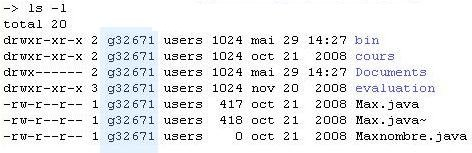
\includegraphics[width=0.8\linewidth,height=0.8\textheight,keepaspectratio=true]{/home/oxfam/Bureau/DEV1ARefaire/labo-cli-02/labo-cli-02/image/ls-l.jpg}
			
		\end{center}
		
		\caption[Contenu d\'etaill\'e d'un dossier]{Contenu d\'etaill\'e d'un dossier}
	\end{figure}
	
	Est-ce qu'un professeur peut l'\'editer ? 
	
%	\par
	\fcolorbox{gray}{verylightgray}{\parbox{\textwidth}{\textcolor{verylightgray}{\LARGE  Non ! Le droit d'écriture n'est accordé qu'au propriétaire.  }}} {\footnotesize\emph{}\par} 
	%(la r\'eponse est disponible dans la version en ligne)
\end{Exercice}	

	
\begin{Exercice}{D\'eterminez les bonnes permissions}	
	           %     \textcolor{white}{.} %\par	
	Soit le fichier "Max.java" de la capture d'\'ecran ci-dessus.
	
	On voudrait que l'\'etudiant g32671 puisse travailler  
	normalement, que les autres \'etudiants ne puissent pas tricher sur  
	lui mais que les professeurs puissent lire son travail.   
	
	\begin{itemize}
		
		\item 
		Quel groupe faut-il donner au fichier ?
		\par
		\textcolor{gray}{\underline{\hspace*{10em}}} 
		\item 
		Quelle commande permet de donner ce groupe au fichier ?
		\par
		\textcolor{gray}{\underline{\hspace*{3em}}}  \textcolor{gray}{\underline{\hspace*{10em}}}  \textcolor{gray}{\underline{\hspace*{10em}}} 
		\item 
		Quelles permissions minimales donner au fichier ?                
		\par
		\textcolor{gray}{\underline{\hspace*{1em}}}  \textcolor{gray}{\underline{\hspace*{1em}}}  \textcolor{gray}{\underline{\hspace*{1em}}}  \textcolor{gray}{\underline{\hspace*{1em}}}  \textcolor{gray}{\underline{\hspace*{1em}}}  \textcolor{gray}{\underline{\hspace*{1em}}}  \textcolor{gray}{\underline{\hspace*{1em}}}  \textcolor{gray}{\underline{\hspace*{1em}}}  \textcolor{gray}{\underline{\hspace*{1em}}} 
		\item 
		Quelle commande permet de donner ces permissions au fichier ?
		\par
		\textcolor{gray}{\underline{\hspace*{3em}}}  \textcolor{gray}{\underline{\hspace*{2em}}}  \textcolor{gray}{\underline{\hspace*{10em}}} 
	\end{itemize}
	
	
\end{Exercice}


\begin{Exercice}{} 
	Reprenez les permissions affich\'ees dans la capture d'\'ecran ci-dessous 
et exprimez-les avec un nombre de 3 chiffres.  

\par
\begin{figure}[hbt]
	\begin{center}
		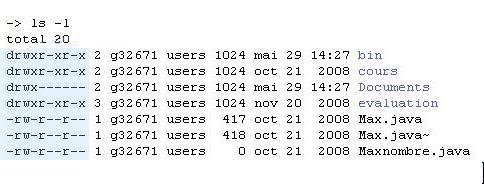
\includegraphics[width=0.8\linewidth,height=0.8\textheight,keepaspectratio=true]{/home/oxfam/Bureau/DEV1ARefaire/labo-cli-02/labo-cli-02/image/ls-l-permissions.jpg}
		
	\end{center}
	
	\caption[Contenu d\'etaill\'e d'un dossier]{Contenu d\'etaill\'e d'un dossier}
\end{figure}
\end{Exercice}
		
		
\begin{Tutoriel}{Permissions par d\'efaut} 	
	%	\textcolor{white}{.} \par
		
	%	\par	
		\begin{enumerate}
			
			\item Si ce n'est pas encore fait, cr\'eez un dossier "td2".
			\item Cr\'eez-y un fichier vide.
			\item Demandez les d\'etails du fichier (propri\'etaire, groupe, permission)
		\end{enumerate}
		
		On constate qu'un nouveau fichier appartient \`a celui qui l'a cr\'e\'e 
		(on s'en doute) et au groupe principal du cr\'eateur. 
		Il y a aussi des permissions par d\'efaut (plut\^ot permissives dans notre cas).  
		
		\par
\end{Tutoriel}		
		
		\subparagraph{Modifier les permissions} 

\textcolor{white}{.} \par

\par

Vous savez que la commande qui permet de modifier les permissions d'un fichier est 
\,\verb|chmod|\,.  

\par

Prenez le temps de \textbf{lire} 
la page de \textbf{manuel} de cette commande.   

\par
	
	\begin{Tutoriel}{Modifier les permissions} 
\begin{enumerate}	
	\item Cr\'eez un fichier "brol" dans le dossier "td2" avec quelques mots.
	\item Faites en sorte que personne d'autre ne puisse en voir le contenu.
	\item Faites en sorte que tout le monde puisse voir son contenu mais pas le modifier. 
	\item 
	Faites en sorte que les autres \'etudiants ne puissent pas voir son contenu mais les professeurs bien. 
	Attention, pour ce faire, il faut pouvoir distinguer les \'etudiants des enseignants; et donc, distinguer les groupes.
	
\end{enumerate}
		
	\end{Tutoriel}

	\begin{Tutoriel}{Modifier encore les permissions}           
Modifiez les droits de votre dossier "td2" et, si n\'ecessaire, 
des fichiers qui s'y trouvent pour que tout le monde puisse  
%\par
\begin{enumerate}
	
	\item voir quels fichiers s'y trouvent mais sans pouvoir lire le contenu de ces fichiers;
	\item modifier le contenu d'un des fichiers mais pas supprimer ce fichier;
	\item supprimer un fichier mais pas modifier son contenu.
\end{enumerate}
	
\end{Tutoriel}


		\subparagraph{FAQ} 

\textcolor{white}{.} \par

\par
\textbf{Pourquoi avoir choisi 4, 2 et 1 pour d\'esigner les permissions ?}
\par

C'est li\'e au code binaire. 'rwx' donne, pour 'r', la valeur '100' soit 4 en d\'ecimal.  

\par
\textbf{Vous dites que dans un affichage en format long, 
	le premier caract\`ere indique si c'est un fichier simple ('-') ou un dossier ('d'). 
	Pourtant j'ai d\'ej\`a vu d'autres symboles. C'\'etait quoi ?
}
\par

Il existe d'autres types de fichiers que les deux que nous avons vus. 
Ils se rencontrent moins souvent et sont surtout utilis\'es par le syst\`eme.
Par exemple, certains d\'efinissent des \textit{pilotes} vers le mat\'eriel. 
Si vous voulez en savoir plus, vous pouvez lire
ceci (\url{en.wikipedia.org/wiki/Unix\_file\_types}).  

\par
\textbf{Vous avez mentionn\'e les permissions 'r', 'w' et 'x'. 
	Pourtant j'ai d\'ej\`a vu d'autres lettres dans la zone r\'eserv\'ee aux permissions. 
	C'\'etait quoi ?
}
\par

Il y a 3 permissions dont nous n'avons pas parl\'e parce qu'elles sont moins courantes : 
le \textit{suid} (set user id), 
le \textit{sgid} (set group id) 
et le \textit{sticky}. 
Si vous voulez en savoir plus, vous pouvez lire   
ceci (\url{fr.wikipedia.org/wiki/Permissions\_UNIX}).  

\par
\textbf{Vous n'avez pas expliqu\'e le sens de la 2\textsuperscript{e} colonne 
	fournie par la commande ls (juste avant le propri\'etaire) ?
}
\par

C'est vrai mais c'est moins utile et plus li\'e \`a la structure interne du syst\`eme de fichier. 
Je veux bien vous dire qu'il s'agit du nombre de liens physiques sur le fichier 
mais je sens que vous commencez d\'ej\`a \`a regretter d'avoir pos\'e la question ;)  

\par
\textbf{Nous avons vu qu'un fichier est cr\'e\'e avec des permissions par d\'efaut. 
	C'est configurable ?
}
\par

Oui. Voyez la commande \,\verb|umask|\,.  

\par
\subsection{Recherche d'informations}  
Non seulement, il y a beaucoup de commandes \`a connaitre mais en plus, chacune dispose d'une multitude d'options. 
Impossible de tout retenir ! Comment faire pour retrouver l'information ?   

\par
\textbf{Si vous connaissez le nom de la commande}
\par
\textit{Solution 1} : Vous pouvez entrer la commande avec l'option \,\verb|--help|\,
qui affiche une aide succinte sur l'utilisation de la commande.
La  plupart des commandes comprennent cette option mais \textbf{pas toutes}.   

\par

\begin{Exemple}{}
	ls --help
\end{Exemple}
%Exemple: \,\verb|ls --help|\,
\par
\textit{Solution 2} : Pour une information plus compl\`ete, il existe la commande \,\verb|man|\,.  

\par

\begin{Exemple}{}
	man ls (\textit{q} pour quitter le man)  
\end{Exemple}
%Exemple: \,\verb|man ls|\,  (\textit{q} pour quitter le man)  

\par
\textbf{Si vous n'avez toujours pas trouv\'e}
\par

Consultez les documents que l'on met \`a votre disposition 
(lien "\textit{Aide}" sur le site).
Notamment notre aide-m\'emoire qui reprend une liste des commandes les plus fr\'equentes 
ou encore le \textit{quick reference} 
qui reprend la plupart des commandes linux sur une feuille recto-verso.  

\par

\begin{Exercice}{} 
	La commande \,\verb|ls -l|\, 
	affiche le contenu du dossier en format \textit{long}.
	Nous verrons plus tard comment comprendre toute cette information 
	mais sachez d\'ej\`a que la 4\`eme colonne donne la taille du fichier (en octets).
	Lorsque les nombres sont grands, ce n'est pas tr\`es lisible. 
	Trouvez l'option qui permet d'afficher cette taille sous un format plus lisible.  
	
	\par
	\textbf{Consigne} : de gr\^ace, 
	\textbf{cherchez} la r\'eponse, 
	ne la \textbf{demandez pas} \`a votre voisin. 
	Le but de cet exercice n'est pas de connaitre l'option 
	(elle n'est pas si utile que \c ca) 
	mais d'apprendre \`a trouver soi-m\^eme l'information.  
	
	\par	
\end{Exercice}


\begin{Exercice}{}
Comment visualiser en une fois tous les fichiers de votre dossier 
mais aussi les fichiers des dossiers qui s'y trouvent et ainsi de suite ? 
(\textbf{r\'ecursivement} en somme)\par

Aide: examinez les options de la commande \,\verb|ls|\,  
Quelle commande permet de \textit{nettoyer} l'\'ecran ?  

\par
	
\end{Exercice}

        \subsection{Conclusion}

\subparagraph{FAQ} 

\textcolor{white}{.} %\par

\par
\textbf{Euh ! Je n'ai pas fini. C'est normal ?}
%\par
Non, c'est que vous avez mal pr\'epar\'e votre TD avant de venir au labo. 
Terminez-le en rem\'ediation et/ou \`a la maison car la semaine prochaine, 
nous en attaquons un nouveau et, cette fois, essayez de mieux vous y pr\'eparer!  

\par
\textbf{Je n'ai pas Linux \`a la maison. Je peux quand m\^eme terminer mon TD ?}
\par

Non. Vous devrez rapidement disposer d'un Linux fonctionnel \`a la maison.
Ce qui devrait d'ailleurs \^etre le cas si vous avez fait
les exercices demand\'es au cours d'introduction \`a l'OS.

\par
\textbf{J'ai un Linux \`a la maison et les groupes ne sont pas les m\^emes. C'est normal ?}
\par

Oui. 
Les groupes d\'ependent \`a la fois de la distribution particuli\`ere utilis\'ee
et de la fa\c con dont l'administrateur (le root) a configur\'e le syst\`eme.   

\par

\end{document}

	
%\clearpage

%%%%%%%%%%%%%%%%%%%%%%%%%%%%%%%%%%%%%%%%%%%%

%C------------------------es exercices pr\'eparatoires sont compos\'es de deux parties :
%
%\par
%
%\begin{itemize}
%	
%	\item quelques questions pour v\'erifier ce que vous avez retenu du TD1;
%	\item les diff\'erents points des documents th\'eoriques \`a lire avant d'aller au laboratoire.
%\end{itemize}
%
%%====================
%%\subsection{Consignes}
%\subsection{Révision du TD1}
%%====================
%\begin{Exercice}{La connexion}
%
%
%Remplissez les blancs.
%
%Nous allons faire les laboratoires sur une machine
%qui se nomme  \textcolor{gray}{\underline{\hspace*{5em}}}  
%et qui tourne sur le syst\`eme d'exploitation        
%\textcolor{gray}{\underline{\hspace*{3em}}} . 
%Pour s'y connecter, nous utilisons le programme Windows        
%\textcolor{gray}{\underline{\hspace*{3em}}} . 
%Nous communiquerons avec la machine en mode  
%\textcolor{gray}{\underline{\hspace*{5em}}}  
%gr\^ace \`a un  \textcolor{gray}{\underline{\hspace*{3em}}}  
%qui se nomme  \textcolor{gray}{\underline{\hspace*{3em}}} . 
%		
%\end{Exercice}
%
%
%
%\begin{Exercice}{Les commandes de base}
%Voyons voir si vous vous rappelez des quelques commandes de base vues la semaine pass\'ee.
%La commande pour :  
%
%\begin{itemize}
%	
%	\item voir le contenu d'un dossier (la liste de ce qu'il contient) est  \textcolor{gray}{\underline{\hspace*{2em}}} 
%	\item \'editer le contenu d'un fichier est  \textcolor{gray}{\underline{\hspace*{3em}}} 
%	\item changer son mot de passe est  \textcolor{gray}{\underline{\hspace*{5em}}} 
%	\item se d\'econnecter de linux1 est  \textcolor{gray}{\underline{\hspace*{3em}}} 
%	\item copier un fichier est  \textcolor{gray}{\underline{\hspace*{2em}}} 
%	\item renommer un fichier est  \textcolor{gray}{\underline{\hspace*{2em}}} 
%	\item d\'eplacer un fichier est  \textcolor{gray}{\underline{\hspace*{2em}}} 
%	\item changer de dossier courant est  \textcolor{gray}{\underline{\hspace*{2em}}} 
%	\item cr\'eer un r\'epertoire est  \textcolor{gray}{\underline{\hspace*{3em}}} 
%	\item visualiser le contenu d'un fichier sans l'\'editer est  \textcolor{gray}{\underline{\hspace*{2em}}} 
%	\item voir quel est le dossier courant (son chemin) est  \textcolor{gray}{\underline{\hspace*{2em}}} 
%	\item d\'etruire un fichier est  \textcolor{gray}{\underline{\hspace*{2em}}} 
%	\item d\'etruire un dossier vide est  \textcolor{gray}{\underline{\hspace*{3em}}} 
%\end{itemize}
%
%\end{Exercice}
%
%
%
%\begin{Exercice}{La ligne de commande}
%					\begin{itemize}
%	
%	\item 
%	Qu'est-ce qui permet de distinguer / s\'eparer les diff\'erentes parties d'une commande ? 
%	\textcolor{gray}{\underline{\hspace*{10em}}} 
%	\item 
%	Dans la commande \,\verb|nanotest|\,, combien y a-t-il de parties ?  
%	\textcolor{gray}{\underline{\hspace*{1em}}} 
%\end{itemize}	
%	
%\end{Exercice}
%
%\clearpage
%%====================
%\subsection{Th\'eorie \`a revoir}
%%====================
%
%						Avant de venir au prochain labo, lisez \textbf{attentivement}
%les points 10 \`a 19 du guide visuel. 
%
%\subparagraph{Choix multiples}
%\textcolor{white}{.} \par
%\begin{Exercice}{Raccourci}
%	Le raccourci qui d\'esigne la home de l'utilisateur \textit{g12345} est
%	
%	\begin{steps} 
%		
%		\item .
%		
%		\item \char`\~
%		
%		\item \char`\~g12345
%		
%		\item /
%		
%		\item /home
%		
%	\end{steps} 
%\end{Exercice}
%
%	
%	
%	\begin{Exercice}{Racine}
%		La racine du syst\`eme de fichier sous Linux est
%		\begin{steps} 
%			\item .
%			
%			\item \char`\~
%			
%			\item \char`\~g12345
%			
%			\item /
%			
%			\item /home
%			
%	\end{steps} 
%\end{Exercice}	
%		
%		
%		\begin{Exercice}{Chemin absolu}
%		            \begin{steps} 
%			
%			\item /home/g54321/td2Prepa
%			
%			\item \char`\~g54321/td2Prepa
%			
%			\item g54321/td2Prepa
%			
%			\item td2Prepa
%			
%		\end{steps} 	
%		\end{Exercice}
%	
%		\begin{Exercice}{Chemin relatif}
%		\begin{steps}
%		            \item td2Prepa
%		
%		\item ../td2Prepa
%		
%		\item ./.././eCours/td2Prepa
%		
%		\item /eCours/java/tds/td2Prepa
%	\end{steps} 
%		\end{Exercice}
%
%		\begin{Exercice}{Permissions}
%	\begin{steps}
%		            \item chmod
%		
%		\item chgrp
%		
%		\item chown
%	\end{steps} 
%		\end{Exercice}
%
%
%
%		
%			
	%%%%%%%%%%%%%%%%%%%%%%%%%%%%%%%%%%%%%%%%%%%%%%
%
%Quelques conseils pour bien travailler et progresser.
%\par
%\begin{itemize}
%\item Faites bien tous les exercices proposés.
%\item Vous pouvez \textbf{coopérer} avec vos condisciples mais nous vous demandons de ne \textbf{pas copier} les réponses. Si vous voulez progresser, \textbf{chercher} la réponse est plus important que de la trouver. 
%\item N'hésitez pas à \textbf{montrer votre travail} à votre professeur.
%\item N'hésitez pas à \textbf{poser des questions} si vous n'avez pas bien compris ce qu'on vous demande.
%\item \textbf{Prenez des notes} ! Ce que vous allez apprendre aujourd'hui vous servira les semaines prochaines mais vous en aurez oublié une grande partie si vous ne notez rien. Le plus pratique est probablement d'annoter la version \textbf{papier}. Nous vous expliquons plus loin comment l'imprimer si ce n'est pas déjà fait.
%\end{itemize}
%%====================
%\subsection{Ressources}
%%=====================
%Nous avons rassemblé sur le site (\textbf{suivez le lien "Aide"}), une série de documents qui peuvent être utiles. Voyez notamment :
%\par
%\begin{itemize}
%\item un \textbf{guide visuel Linux} : document écrit par nos soins qui explique de façon simple et visuelle les bases de Linux. Vous pouvez le consulter quand vous n'avez pas \textbf{compris} un point de matière. Certains points sont à lire \textbf{avant} de venir au laboratoire ;
%\item un \textbf{aide-mémoire} : document écrit par nos soins sur l'utilisation de Windows et Linux. Vous pouvez le consulter quand vous avez \textbf{oublié} quelque chose (le nom d'une commande, une procédure...) ;
%\item	un \textbf{quick reference Linux} : reprend, en condensé, toutes les commandes Linux les plus utiles. 
%\end{itemize}
%
%
%%===================
%\section{Windows}
%%====================
%
%Comme vous avez pu le constater, les PC des laboratoires sont équipés du système \verb_Windows_.
%\par			
%Au laboratoire, vous vous connecterez sur un serveur \verb_Linux_. Windows vous servira essentiellement à : vous connecter au Linux, 
%effectuer des recherches sur Internet, imprimer et transférer des fichiers.
%\par
%Si vous avez une question concernant l'utilisation de Windows vous trouverez peut-être la réponse dans l'aide-mémoire que nous avons déjà cité dans la partie "ressources". Il est disponible sur poÉSI et vous y trouverez par exemple des explications sur l'impression.
%\par			
%		
%
%%====================
%\subsection{Imprimer}
%%====================
%Si vous voulez imprimer ce TD (ce qui est une bonne idée), vous devez \textit{installer} une imprimante. Vous trouverez comment faire en consultant l'aide-mémoire sur poÉSI.
%\par
%%====================
%\subsection{Changer le mot de passe sous Windows}
%%=====================
%
%
%\subparagraph{Réflexion}
%\textcolor{white}{.} 
%\par
%				
%\`A votre avis, pourquoi vous demande-t-on de modifier votre mot de passe ?
%				
%\par
%{\footnotesize\emph{(la r\'eponse est disponible dans la version en ligne)}\par} 
%			
%%\subparagraph{Exemples de mots de passe} 
%\begin{Exercice}{Exemples de mots de passe} 		
%%\textcolor{white}{.} 
%%\par
%Quelles sont les propositions qui vous paraissent correctes comme mot de passe ?
%\begin{itemize} 
%  \item[ \ding{"6F} ] nadia
%  \item[ \ding{"6F} ] M0nAm1eN@di@
%  \item[ \ding{"6F} ] m@C0p1ne
%  \item[ \ding{"6F} ] GH5).jg
% \end{itemize} 
%\end{Exercice} 
% 
%\subparagraph{Changer le mot de passe} 
%		
%\textcolor{white}{.} 
%\par
%				
%\par
%        
%Il est  temps de \textbf{changer votre mot de passe}. Consultez l'aide-m\'emoire si vous ne savez pas comment faire. 
%				
%\par
%        
%			
%\subparagraph{FAQ Windows} 
%		
%\textcolor{white}{.} \par
%				
% \par
% \textbf{Je ne suis pas content du mot de passe que j'ai choisi. Est-ce que je peux le changer ?}
% \par
%Oui mais pas tout de suite. L'administrateur des machines Windows de l'\'ecole impose un temps minimum (1 jour) entre 2 modifications de mot de passe.
% \par
% \textbf{Est-ce que je vais pouvoir garder ce mot de passe toute l'ann\'ee ?}
%\par
%Non. Pour des raisons de s\'ecurit\'e, Windows va vous demander de changer le mot de passe d'ici quelques mois.
%\par
% \textbf{J'ai oubli\'e mon mot de passe. Qu'est-ce que je peux faire ?}
% \par
% Les professeurs ne peuvent ni retrouver votre nouveau mot de passe, ni remettre le mot de passe de d\'epart. Par contre le technicien (F. Marchal qui a son bureau au 5\textsuperscript{\`eme}) peut remettre le mot de passe de d\'epart. Allez le trouver (et prenez garde \`a ce que \c ca n'arrive plus !)
% \par
%
%\clearpage
%%===================
%\section{Linux}
%%====================
%\begin{quotation}
%\guillemotleft  \textit{Linux ? Il y a moins bien mais c'est plus cher} \guillemotright . Auteur inconnu
%\end{quotation}
%%====================
%\subsection{Présentation}
%%====================
%Vous ne travaillerez pas directement sur votre PC durant les laboratoires Java. Celui-ci vous servira pour vous connecter au serveur Linux (son nom est \verb_linux1_)
% \par
% \textbf{Tiens, c'est quoi Linux et pourquoi l'utiliser ? C'est quoi une machine partag\'ee?}
% \par
%  Si vous vous posez ce genre de questions (et c'est bien !), je vous invite vivement \`a (re)lire le point 1 du guide visuel (cf. documents d'aide).
% \par
%%====================
%\subsection{Se connecter}
%%=====================
%Lorsque vous allez vous connecter, \verb_linux1_ va vous demander de vous identifier.
%				
% \par
%        
%\begin{itemize}
%				
%\item Votre \textbf{\textit{username}} est le m\^eme que sous Windows (avec un \textbf{'g' minuscule} obligatoirement ; ex:	\verb_g32010_).
%\par
%\textbf{Note} : pour Linux, les minuscules et les majuscules sont toujours des caract\`eres diff\'erents.
%					
%\item Votre \textit{\textbf{mot de passe}} est le m\^eme que votre \textbf{mot de passe initial sous Windows}.
%					
%\end{itemize}
%				
%Le mot de passe sous Windows et sous Linux sont 2 mots de passe diff\'erents (initialis\'es \`a la m\^eme valeur).
%        
%\par
%        
%Vous avez modifi\'e votre mot de passe sous Windows mais pas encore sous Linux (vous le ferez plus tard...)
%				
%\par
%%\subparagraph{Connectez-vous \`a linux1} 
%\begin{Tutoriel}{Connectez-vous \`a linux1} 
%		
%\textcolor{white}{.} \par
%				
% \par
% \begin{figure}[hbt]      
% \begin{coltbox}{Attention}
%Seulement les images peuvent \^etre repr\'esent\'ees dans cette version! Flash, animation, son etc. sont visibles uniquement dans la version en ligne.
%\end{coltbox}
%%\end{fhint}
%\caption[PuTTY.mov]{PuTTY.mov}
%\end{figure}
%				
%\par
%Il y a 4 \'etapes :
%\par
%        
%\begin{steps}
%				
%\item lancez l'application \verb_putty_ (vous la trouverez dans le menu ou comme raccourci sur le bureau) ;
%					
%\item indiquez \`a \verb_putty_ le nom de la machine (\textit{Host Name}) \`a laquelle vous voulez vous connecter (ici \verb_linux1_) ;
%{\footnotesize\emph{(une capture d'\'ecran est disponible dans la version en ligne)}\par} 
%
%\item cliquez sur "\textbf{Open}" ; la connexion se fait ! S'il vous pr\'esente une boite de message avec un "\textbf{Security Alert}", cliquez sur "\textbf{Yes}" en toute confiance ;
%					
%\item identifiez-vous !
%						
%\begin{steps}
%\item Tapez votre nom d'utilisateur (\,\verb|gxxxxx|\,) puis sur la touche \,\verb|ENTREE|\,.\par 
%\textbf{Note} : Soyez attentif au g\,\verb|g|\, minuscule.
%
%\item Tapez votre mot de passe puis sur la touche \,\verb|ENTREE|\,.\par
%\textbf{Note} : Rien ne s'affiche quand vous tapez votre mot de passe ; c'est normal.
%\end{steps}
%\end{steps}
%\end{Tutoriel}		       
%
%%====================
%\subsection{Le mode console}
%%=====================
%Si vous ne voyez pas du tout ce qu'est le mode console ou comment entrer une commande, allez d'abord faire un petit tour aux points 2 et 3 du guide visuel.
%				
%\par
%        
%\subparagraph{Ma premi\`ere commande} 
%\textcolor{white}{.} \par	
%\begin{steps}
%\item Entrez la commande \,\verb|ls|\, (n'oubliez pas la touche \,\verb|ENTREE|\,).
%\end{steps}				
%\par
%        
%Vous constatez que le bash a affich\'e quelque chose (d'incompr\'ehensible pour le moment ; ne vous inqui\'etez pas nous y reviendrons) et qu'il vous propose \`a nouveau l'invite de commande.
%				
%\par
%        
%			
%\subparagraph{Il faut \^etre pr\'ecis !} 
%\textcolor{white}{.} \par
%\begin{steps}
%\item Entrez \`a pr\'esent  la commande \,\verb|LS|\,.
%\end{steps}
%				
%\par
%        
%Vous voyez que le r\'esultat est diff\'erent : il ne comprend pas ce que vous lui voulez.
%        
%\par
%        
%En Linux, \textbf{les majuscules et les minuscules n'ont pas le m\^eme sens, vous devez respecter la casse.}
%\par
%        
%Faites une autre exp\'erience. 
%        
%\par
%        
%Tapez les 3 commandes suivantes qui ne se diff\'erencient que par la pr\'esence ou non d'espaces.
%				
%\par
%        
%\begin{steps}
%				
%\item \,\verb|ls /home|\,
%\item \,\verb|ls/home|\,
%\item \,\verb|ls / home|\,
%
%\end{steps}
%				
%\`A nouveau le r\'esultat est diff\'erent dans les 3 cas. \textbf{Les espaces ont de l'importance}.
%				
%\par
%
%%====================
%\subsection{Changer le mot de passe sous Linux}
%%=====================
%La commande pour changer le mot de passe est \,\verb|passwd|\,.
%				
% \par
%        
%\begin{itemize}
%				
%\item Les r\`egles \`a respecter sont quasiment les m\^emes que sur Windows. Attention toutefois \`a ne pas choisir un mot du dictionnaire.
%\item Vous pouvez d'ailleurs reprendre le m\^eme mot de passe que celui que vous avez choisi pour Windows. Mais contrairement \`a celui sous Windows, le mot de passe Linux pourra \^etre conserv\'e toute l'ann\'ee.
%					
%\end{itemize}
%				
%			
%\subparagraph{\`A vous !} 
%		
%\textcolor{white}{.} \par
%				
% \par
%        
%Tapez la commande ad\'equate pour changer votre mot de passe.
%				
%\par
%        
%\begin{itemize}
%				
%\item Le syst\`eme vous demande de taper le mot de passe actuel (vous ne le voyez pas quand vous le tapez, c'est normal !)
%\item Ensuite, vous entrez le nouveau mot de passe que vous venez de choisir.
%\item Vous retapez une deuxi\`eme fois ce mot de passe pour le confirmer.
%
%\end{itemize}
%\textbf{Si \c ca va mal...}
%\par
%        
%\begin{itemize}
%				
%\item \textit{Quand je tape la commande rien ne se passe !}
%
%\begin{itemize}				
%\item Avez-vous bien appuy\'e sur la touche \,\verb|ENTREE|\, ?
%\item Une seule personne \`a la fois peut changer son mot de passe et vous \^etes tous connect\'es \`a la m\^eme machine. Soyez patient.
%\end{itemize}
%				
%\item \textit{Apr\`es avoir tout entr\'e, il me met un message d'erreur !}
%\begin{itemize}
%\item \textbf{Lisez le message} ! Il est en g\'en\'eral assez explicite.
%\item Peut-\^etre que le mot de passe est trop simple.
%\item Peut-\^etre n'avez-vous pas respect\'e les minuscules/majuscules.
%\end{itemize}
%\end{itemize}
%				
%			
%\subparagraph{V\'erification} 
%		
%\textcolor{white}{.} \par
%				
%\par
%        
%Pour v\'erifier que tout s'est bien pass\'e, vous pouvez vous d\'econnecter et vous reconnecter.
%        
% \par
%        
%Pour quitter proprement \verb_linux1_, la commande est \,\verb|exit|\,.
%				
%\par
%
%%====================
%\subsection{Le dossier personnel et le dossier courant}
%%=====================
%Un petit tour pr\'ealable aux points 4 \`a 7 du guide visuel est vivement conseill\'e.
%				
% \par
%        
%			
%\subparagraph{Examiner son dossier} 
%		
%\textcolor{white}{.} \par
%				
%\par
%        
%Comment voir le contenu de votre dossier ? Simplement avec la commande\,\verb|ls|\, que vous avez d\'ej\`a rencontr\'ee.
%				
%\par
%
%%\subparagraph{Exp\'erimentation} 
%\begin{Tutoriel}{Exp\'erimentation}  
%\begin{steps}
%\item Tapez la commande \,\verb|ls|\,.
%\end{steps}				
%\par
%        
%\begin{itemize}
%\item Il vous montre le contenu de votre dossier.
%\item Vous constatez qu'il contient d\'ej\`a des \'el\'ements.
%\item La couleur permet de distinguer un dossier (en bleu) d'un fichier (en blanc).
%\item Comme sur Windows, la notion de dossier est hi\'erarchique : un dossier peut contenir des fichiers mais aussi d'autres dossiers qui \`a leur tour...
%\end{itemize}
%				
%\begin{steps}
%\item Tapez la commande \,\verb|ls bin|\,.
%\end{steps}
%				
%\par
%\begin{itemize}
%\item Cette fois, il vous montre le contenu du dossier \textit{bin} (ne vous inqui\'etez pas, la commande n'affiche rien parce que le dossier est vide).
%\end{itemize}
%\begin{steps}
%\item	 \`A pr\'esent, tapez la commande \,\verb|cd bin|\,.
%\end{steps}				
%\par
%        
%\begin{itemize}
%\item Cette commande demande de se \textit{\textbf{d\'eplacer}} dans le dossier \textit{bin}.
%\end{itemize}
%\begin{steps}
%\item	Retapez la commande	\,\verb|ls|\, du d\'ebut.
%\end{steps}
% \par
% \begin{itemize}
%\item Le r\'esultat est diff\'erent. Est-ce que vous comprenez pourquoi ?
%\end{itemize}
%\end{Tutoriel}
%\subparagraph{Le dossier courant} 
%		
%\textcolor{white}{.} \par
%				
%\par
%        
%\`A tout moment, vous \^etes \textit{dans} un dossier, appel\'e le \textbf{dossier courant} (\textit{working directory} en anglais).
%				
% \par
%        
%Il est repr\'esent\'e par "\,\verb|.|\,".
%				
%\par
%        
%\begin{itemize}
%\item La commande \,\verb|cd|\, (\textit{change directory}) permet de changer de dossier courant.
%\item La commande \,\verb|cd|\, sans rien derri\`ere vous ram\`ene toujours dans votre dossier personnel.
%\item La commande \,\verb|cd .|\, vous laisse l\`a o\`u vous \^etes, \,\verb|.|\, repr\'esentant votre dossier courant.
%\item La commande \,\verb|cd ..|\, vous am\`ene dans le dossier juste au-dessus de celui o\`u vous \^etes, on parle de \textit{r\'epertoire parent}. \,\verb|..|\, repr\'esente le r\'epertoire parent du r\'epertoire courant.
%\item La commande \,\verb|pwd|\, (\textit{print working directory}) permet d'afficher le chemin du dossier courant (o\`u vous \^etes pour le moment).
%\end{itemize}
%\textbf{C'est quoi le chemin ?}
%\par
%C'est la suite des dossiers qu'il faut traverser. Nous verrons \c ca plus en d\'etail dans le prochain TD.
%				
%\par
%        
%%\subparagraph{Exp\'erimentation} 
%\begin{Tutoriel}{Exp\'erimentation}      
%\begin{steps}
%				
%\item En pr\'eambule, tapez la commande \,\verb|cd|\, pour revenir dans \textit{votre home} (dossier personnel).
%\item Tapez \`a pr\'esent la commande \,\verb|ls bin|\,.
%\item Comparez le r\'esultat avec celui produit par les 2 commandes suivantes : \,\verb|cd bin|\, et \,\verb|ls|\,
%\end{steps}
%\end{Tutoriel}				
%			
%\subparagraph{Question} 
%		
%\textcolor{white}{.} \par
%				
%\par
%Est-ce qu'on peut dire que \,\verb|ls bin|\, est strictement \'equivalent \`a \,\verb|cd bin|\, suivi de \,\verb|ls|\, ?
%				
%\par
% \fcolorbox{gray}{verylightgray}{\parbox{\textwidth}{\textcolor{verylightgray}{\LARGE Non ! Dans le 1 er cas, on ne modifie pas le dossier courant. Dans le 2 ème cas oui. }}}
%  {\footnotesize\emph{(la r\'eponse est disponible dans la version en ligne)}\par} Comment le mettre en \'evidence ?
% \par
% \fcolorbox{gray}{verylightgray}{\parbox{\textwidth}{\textcolor{verylightgray}{\LARGE On peut le mettre en évidence en tapant la commande pwd après chaque cas.}}} 
% {\footnotesize\emph{(la r\'eponse est disponible dans la version en ligne)}\par} 										
%			
%        
%			
%
%
%%====================
%\subsection{L'éditeur}
%%=====================
%
%Un petit tour pr\'ealable au point 8 du guide visuel est vivement conseill\'e.
%				
%\par
%        
%%\subparagraph{Exp\'erimentation} 
% \begin{Tutoriel}{Exp\'erimentation}     
%\begin{steps}
%\item En pr\'eambule, tapez la commande \,\verb|cd|\, pour revenir dans \textit{votre home} (dossier personnel).
%\item Tapez \,\verb|nano test|\, pour commencer \`a \'editer le fichier \verb_test_ (comme il n'existe pas encore, il est cr\'e\'e).
%\item Une fen\^etre s'ouvre. Vous voyez qu'elle est scind\'ee en 2 parties : la partie sup\'erieure o\`u vous \'ecrivez votre texte et la partie inf\'erieure o\`u sont indiqu\'ees les diff\'erentes commandes (le \char`\^ repr\'esente la touche Ctrl)
%\item Entrez quelques mots.
%\item Appuyez sur la combinaison de touches \,\verb|Ctrl X|\,, confirmez que vous voulez sauver vos modifications et sortez.
%\item Vous \^etes maintenant revenu \`a l'invite de commande.
%\item Tapez \`a pr\'esent la commande \,\verb|ls|\,.Vous pouvez constater que le fichier \verb_test_ est apparu dans la liste ;)
%\end{steps}
%\end{Tutoriel}
%%====================
%\subsection{Quelques commandes courantes}
%%=====================
%%\subparagraph{Faisons le point} 
%\begin{Exercice}{Faisons le point}		
% \textcolor{white}{.} \par
%            
%Vous avez d\'ej\`a eu l'occasion d'utiliser 6 commandes : \,\verb|passwd|\,,\,\verb|ls|\,,\,\verb|cd|\,,\,\verb|pwd|\,,\,\verb|exit|\, et \,\verb|nano|\,.
%							
%Voyons voir si vous avez retenu leur signification.
%						
%\begin{itemize}
%\item La commande pour voir le contenu d'un dossier (la liste de ce qu'il contient) est \textcolor{gray}{\underline{\hspace*{2em}}} 
%\item La commande pour \'editer le contenu d'un fichier est \textcolor{gray}{\underline{\hspace*{3em}}} 
%\item La commande pour changer son mot de passe est \textcolor{gray}{\underline{\hspace*{5em}}} 
%\item La commande pour se d\'econnecter de linux1 est \textcolor{gray}{\underline{\hspace*{3em}}} 
%\item La commande pour changer de dossier courant est \textcolor{gray}{\underline{\hspace*{2em}}} 
%\item La commande pour voir le chemin du dossier courant est \textcolor{gray}{\underline{\hspace*{2em}}} 
%\end{itemize}
%\end{Exercice}
%				
%\subparagraph{Quelques commandes en plus...} 
%\textcolor{white}{.} \par
% \par
% Il est temps de voir quelques commandes suppl\'ementaires.
% \par
%        
%\begin{itemize}
%\item \,\verb|cat nomDuFichier|\,
%affiche \`a l'\'ecran le contenu du fichier dont le nom est donn\'e (ce n'est pas un \'editeur, on voit le contenu et c'est tout) ;
%\item \,\verb|mkdir nomDuDossier|\, cr\'ee un dossier (vide) nomm\'e "\textit{nomDuDossier}" ;
%\item \,\verb|mv nomDuFichier nouveauNomDeFichier|\, renomme le fichier donn\'e "\textit{nomDuFichier}" sous le nom "\textit{nouveauNomDeFichier}" ;
%\item \,\verb|mv nomDuFichier nomDuDossier|\, d\'eplace le fichier donn\'e dans le dossier indiqu\'e ;
%\item \,\verb|cp nomDuFichier nouveauNomDeFichier|\, cr\'ee une copie du fichier sous le nom "\textit{nouveauNomDeFichier}" ;
%\item \,\verb|cp nomDuFichier nomDuDossier|\, copie le fichier donn\'e dans le dossier indiqu\'e ;
%\item \,\verb|rm nomDuFichier|\, d\'etruit le fichier dont on donne le nom ;
%\item \,\verb|rmdir nomDuDossier|\, d\'etruit le dossier dont on donne le nom (Attention, le dossier doit \^etre vide !).
%\end{itemize}
%
%
%
%\begin{Exercice}{}
%Cr\'eez un dossier \verb_td1_ et d\'eplacez-y le fichier \verb_test_ que vous avez d\'ej\`a cr\'e\'e.
%\textbf{Rappel} : Notez bien votre r\'eponse. Il est difficile de tout retenir la premi\`ere fois; vous serez bien content en relisant vos notes de pouvoir retrouver comment vous avez fait !
%\end{Exercice}	
%		
%\begin{Exercice}{}
%\begin{enumerate}
%\item Prenez une copie de votre fichier \verb_test_ (appelez-la \verb_test2_).
%\item \'Editez ce fichier et ajoutez-y quelques mots.
%\item Affichez le contenu des 2 fichiers pour v\'erifier qu'ils sont bien diff\'erents.
%\end{enumerate}
%\end{Exercice}
%				
%\begin{Exercice}{}
%\begin{enumerate}
%\item Cr\'eez, dans votre dossier \verb_td1_, un dossier \verb_monDossier_.
%\item D\'eplacez-y votre fichier \verb_test2_.
%\end{enumerate}
%\end{Exercice}	
%
%\begin{Exercice}{}
%D\'etruisez le dossier \verb_monDossier_ (ainsi que son contenu).
%\end{Exercice}	
%
%%====================
%\subsection{La ligne de commande}
%%=====================
%Nous avons d\'ej\`a parl\'e de la ligne de commande mais il reste un \'el\'ement dont nous n'avons pas parl\'e, les \textbf{options} :  
%				
% \par
%\begin{itemize}
%\item une option modifie le sens d'une commande ;
%\item elle commence par le signe "\verb|-|" suivi d'une seule lettre ;
%\item ou encore par le double tiret "\verb|--|" suivi d'un nom d'option.
%\end{itemize}
%				
%Les options sont plac\'ees n'importe o\`u apr\`es le nom de la commande.   
%				
%\par
%        
%			
%%\subparagraph{Exp\'erience} 
%\begin{Tutoriel}{Exp\'erimentation}		
%\textcolor{white}{.} \par
%				
% \par
%        
%\begin{steps}
%\item Tapez la commande \,\verb|ls -l|\,. Vous constatez que le r\'esultat obtenu est beaucoup plus verbeux que celui obtenu sans l'option.
%\item Tapez la commande \,\verb|cat -n td1/test|\,. L'option demande de num\'eroter les lignes (note: nous supposons que vous avez bien cr\'e\'e le r\'epertoire \textit{td1} qui contient le fichier \textit{test} lors du labo pr\'ec\'edent et que vous vous trouvez dans \textit{votre home}).
%\item Essayez \,\verb|cat --number td1/test|\,. C'est la version \textit{longue} tout-\`a-fait \'equivalente \`a la pr\'ec\'edente.
%\end{steps}
%\end{Tutoriel}
%%====================
%\subsection{FAQ Linux}
%%=====================
%\textbf{Vous me dites que la commande pour changer le mot de passe est}\,\verb|passwd|\,\textbf{et que celle pour quitter est}\,\verb|exit|\,. \textbf{Je vais devoir retenir tout \c ca ?}
% \par
%Oui ! En tout cas pour les plus fr\'equentes mais l'apprentissage se fera naturellement \`a force de les utiliser.
%						
%\par
% \textbf{Et si j'ai oubli\'e le nom d'une commande ou une option?}
% \par
%         
%Vous verrez la semaine prochaine les moyens mis \`a votre disposition pour retrouver le nom d'une commande ou pour apprendre \`a l'utiliser correctement.
%						
% \par
%\textbf{J'ai quitt\'e en fermant la fen\^etre, ce n'est pas plus simple ?}
%\par
%        
%Oui ! Mais c'est impoli de quitter quelqu'un sans lui dire au revoir ! ;) 
%						
%\par
%Plus s\'erieusement, vous coupez brutalement la conversation avec \verb_linux1_ ce qui peut laisser trainer des programmes actifs et vous emp\^echer de vous connecter la prochaine fois.
%						
%\par
% \textbf{J'ai oubli\'e mon mot de passe. Je dois aussi aller voir F. Marchal ?}
% \par
%        
%Non ! Votre professeur de Java peut r\'einitialiser le mot de passe Linux \`a sa valeur initiale.
%						
% \par
%
%%===================
%\section{Les outils virtuels}
%%====================
%Cette partie d\'epasse un peu le cadre strict des laboratoires Java. Nous voudrions profiter de votre pr\'esence \`a un laboratoire pour vous pr\'esenter les diff\'erents outils virtuels mis \`a votre disposition par l'\'ecole.
%\par
%
%%====================
%\subsection{Les outils virtuels}
%%=====================
%\subparagraph{A. Le site de l'\'ecole} 
%		
%\textcolor{white}{.} \par
%				
%Vous avez probablement d\'ej\`a visit\'e le site web (\url{esi-bru.be}) de l'\'ecole. C'est l\`a que vous trouverez tous les documents officiels.
%			
% \par
%        
%\begin{Exercice}{}
%Allez sur le site de l'\'ecole et retrouvez-y deux documents qui vous seront utiles dans votre parcours scolaire :
%\begin{itemize}
%\item Le calendrier acad\'emique : les dates de cong\'es, d'examens...
%\item Le r\'eglement des \'etudes qui reprend l'ensemble de vos droits et devoirs en tant qu'\'etudiant.
%\end{itemize}
%\end{Exercice}				
%
%        
%\subparagraph{B. po\'ESI} 
%\textcolor{white}{.} \par
%Vous avez d\'ej\`a fait connaissance avec po\'ESI. Cette \textbf{plateforme d'apprentissage en ligne} est l'outil principal utilis\'e dans tous les cours pour mettre toutes les notes \`a disposition des \'etudiants
%			
% \par
% \textbf{Attention !} M\^eme si le syst\`eme de messagerie de po\'ESI envoie une copie par mail, pr\'ef\'erez l'envoi direct d'un mail pour nous contacter. 
%			
% \par
%        
%			
%\subparagraph{C. Le mail} 
%		
%\textcolor{white}{.} \par On vous a d\'ej\`a montr\'e comment utiliser votre messagerie pour connaitre votre mot de passe 
%po\'ESI. 
%			
% \par N'utilisez que cette adresse pour toute communication avec l'\'ecole : professeurs, service administratif...
% \par
%Si vous voulez (sans en abuser), poser une question \`a tous les profs de l'unit\'e d'enseignement DEV1 en un seul mail, vous pouvez (sans en abuser, j'insite) utiliser l'adresse \textit{esi-dev1-list@he2b.be}.
%			
% \par
%        
%\subparagraph{D. Le drive} 
%		
%\textcolor{white}{.} \par
%				
%Vous disposez d'un espace de 30Go dans le cloud, g\'er\'e par Google. Vous pouvez y d\'eposer vos fichiers li\'es \`a l'\'ecole et utiliser tous les services li\'es : partage de document, travail collaboratif... Apprenez \`a l'utiliser !
%			
% \par 
% Pour y acc\'eder, il y a plusieurs possibilit\'es. Si vous \^etes d\'ej\`a connect\'e \`a votre mail, vous pouvez simplement cliquer sur l'ic\^one en haut \`a droite de l'\'ecran. Sinon, vous pouvez vous rendre \`a l'adresse https://drive.google.com (\url{https://drive.google.com}).
%			
% \par
%Pour le moment, cet espace est peu utilis\'e dans les \'echanges \'etudiants-professeurs car nous privil\'egions l'utilisation de \textit{po\'ESI}mais n'h\'esitez pas \`a l'utiliser pour vous et entre vous !
%			
%\par
%\begin{Exercice}{}
%Allez sur votre drive, cr\'eez un dossier \verb_Java_ et, dedans, un fichier texte \verb_Notes_ que vous pourrez utiliser pour prendre quelques notes.
%\end{Exercice}
%
% \par
%        
%\subparagraph{E. L'agenda} 
%		
%\textcolor{white}{.} \par
%Google met \'egalement \`a disposition un agenda. Nous ne l'\textbf{utilisons pas} pour l'instant pour communiquer des dates importantes (cours, interrogations,...) mais vous pouvez l'utiliser pour vous ; il est facilement int\'egrable \`a tout autre syst\`eme d'agenda que vous pourriez d\'ej\`a utiliser.
%			
%\par
%
%%===================
%\section{Conclusion}
%%====================
%%====================
%\subsection{Félicitations}
%%=====================
%Vous \^etes arriv\'es au bout de ce premier TD.
% \par
%Avant de quitter le laboratoire, n'oubliez pas de quitter proprement la connexion avec \verb_linux1_ (\,\verb|exit|\,). et d'\'eteindre l'ordinateur ou de vous d\'eloguer.
%\par
%Attention, afin d'arriver au laboratoire dans les meilleures conditions, il est bien de revoir la mati\`ere qui sera mise en pratique.  C'est pourquoi nous vous fournissons quelques \textbf{exercices pr\'eparatoires} \`a faire \`a la maison pour vous permettre d'\'evaluer si vous \^etes pr\^et.  Afin de v\'erifier que vous pr\'eparez bien ces exercices, des \textbf{interrogations} seront organis\'ees tr\`es r\'eguli\`erement en d\'ebut d'ann\'ee. 
% \par
%\`A la semaine prochaine et soyez \`a l'heure !
%\par
%	
%	
%\end{document}